
Se va a proceder a una exposición del vocabulario utilizado en el diseño del software propio de este marco teórico. Las referencias básicas utilizadas para esta exposición de \gls{DDD} son:

\begin{itemize}
    \item Domain-Driven Design: Tackling Complexity in the Heart of Software.\cite{EricEvans2003DDTC}
    \item Implementing Domain-Driven Design.\cite{VaughnVernon2013IDD}
    \item Get Your Hands Dirty on Clean Architecture\cite{TomHombergs2019GYHD}
\end{itemize}

\textit{DDD} es una metodología de diseño enfocada a desarrollar un lenguaje común para todos los partícipes en un problema y su solución por ejemplo: clientes, vendedores, técnicos y financieros en un programa de gestión de venta de productos. Para desarrollar ese lenguaje se divide el problema en contextos delimitados. En un ejemplo rápido: afiliado en un club deportivo significa facturas, números de identificación fiscal para los financieros y para la gente de operaciones significa reserva de pistas y cancelaciones. Para los de ventas significan descuentos, promociones, los demás actores tendrán otro significado para el mismo concepto. pero cuando hablan de afiliados deben entenderse. Si en un departamento lo llaman clientes y en otro afiliados surgen problemas de comunicación. Tener un lenguaje común donde todos puedan expresarse y hablar de la misma solución es el reto de este proceso. Es lo que se define como \gls{UL} Intentar expresar en un mismo contexto todos esos significados termina en lo que se conoce como "Big Ball of Mud" o Gran bola de barro.


Los componentes y las relaciones de este UL se pueden apreciar en la figura~\cref{fig:DomainDrivenDesignReference}.

\begin{figure}[H]
    \centering
    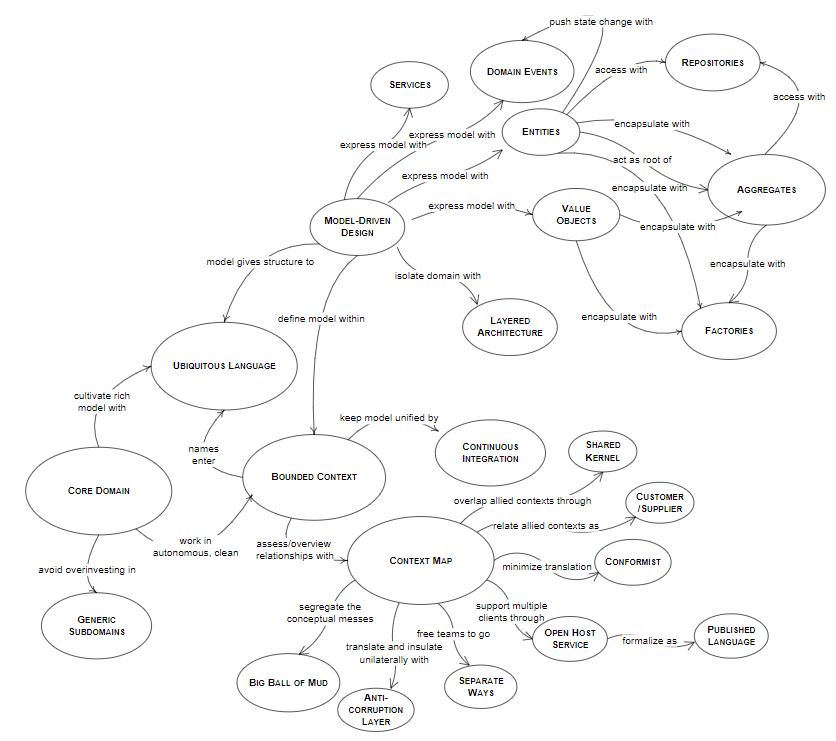
\includegraphics[height=0.5\textheight]{./part/Proyecto_ejecutivo/memoria_descriptiva/infoPreviaAntecedentes/img/DomainDrivenDesignReference}
    \caption{DomainDrivenDesignReference\cite{EricEvans2003DDTC}}\label{fig:DomainDrivenDesignReference}
\end{figure}

De todo este diagrama los conceptos en los que nos vamos a centrar son en los que surgen del componente "Model Driven Design" que son los elementos dentro de ese lenguaje que afectan al diseño del software a su nivel más elemental.

\begin{itemize}
    \item Entity: Elemento que contiene atributos definido por un identificador
    \item \textit{Value Object}: Elemento que tiene atributos pero no identificador
    \item Domain Event: Elemento que define una suceso inducido por la interacción entre los componentes del dominio.
    \item Aggregate: Cluster de elementos tratado como una unidad. Las referencias o acciones externas sobre sus elementos siempre se hacen a través de un único elemento de este cluster conocido como \textit{Agreggate Root}. Tiene reglas definidas de consistencia dentro de su delimitación.
    \item Repository: Es un mecanismo de interaccion para encapsular el acceso a tecnologías, como el almacenamiento en base de datos, para interactuar con ellas. La implementación no concierne al dominio.
    \item Service: Es una funcionalidad de interacción entre elementos de dominio. Encapsula lógica compleja que garantiza un comportamiento consistente.
\end{itemize}

Esta paradigma de diseño compone el elemento central en el paradigma de la arquitectura de capas o \gls{LayerArchitecture}. Se aisla esos contextos que definen nuestro dominio de implementaciones concretas ya sea para acceder al mismo o a las que accede el dominio. Por ejemplo, aislarlo de que se ejecute un servicio mediante una consola de comandos o desde una llamada http y que se guarde en una base de datos la información o se guarde en un archivo.

Dentro de las arquitecturas de capas vamos a utilizar un diseño de puerto y adaptadores o más conocido como \gls{HexagonalArchitecture}. El diagrama básico más utilizado en la teoría para representarlo se muestra en la figura~\cref{fig:hexagonalDiagram}. Como apreciación personal no le encuentro una utilidad real a este tipo de diagramas. El pretendido enfoque didáctico se pierde ya que el hexágono es una simple licencia estética. En el caso de existir más puertos de salida y entrada que los representados, el hexágono pierde todo el sentido. Cuando se enfrenta por primera vez este diagrama se tiende a intentar descifrar el sentído oculto detrás de la elección de la forma poligonal, no existe.

\begin{figure}[H]
    \centering
    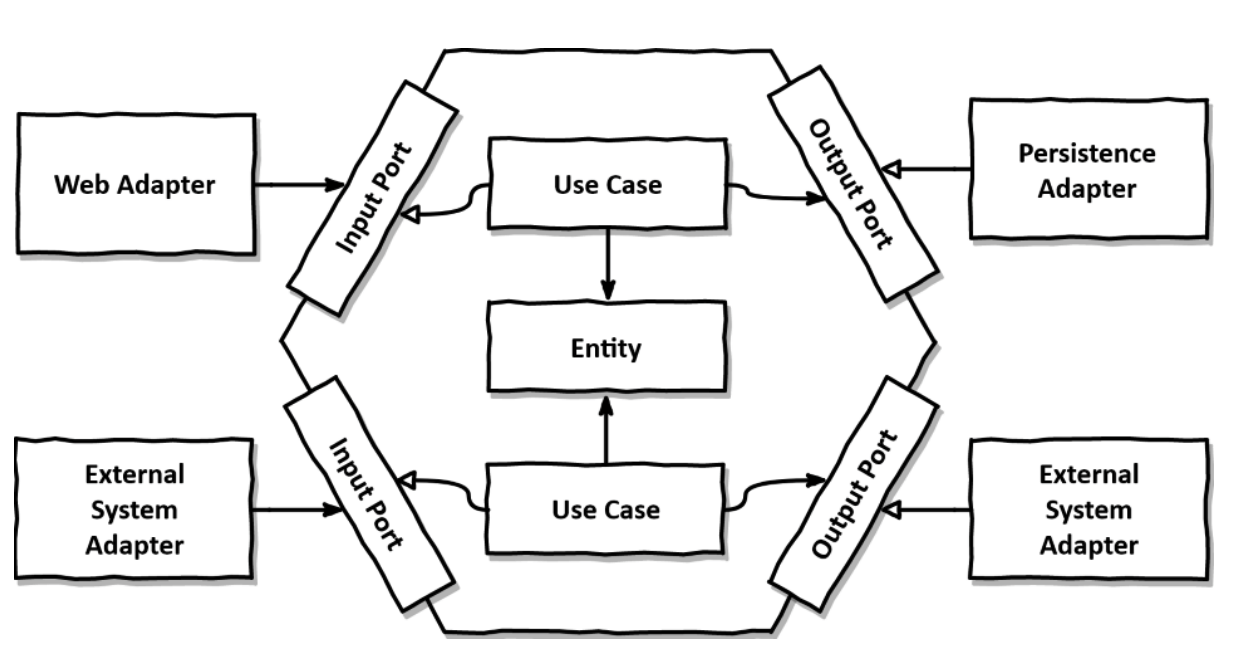
\includegraphics[height=0.3\textheight]{./part/Ejecucion/Seguimiento/CreateTaskUseCase/img/HexagonalDiagram}
    \caption{Hexagonal architecture diagram\cite{TomHombergs2019GYHD}}\label{fig:hexagonalDiagram}
\end{figure}

En este diagrama, el dominio está representado por una única entidad, o Entity, que se encuentra aislada de todo y no depende de ningún elemento. La aplicación está respresentada por los casos de uso, o UseCase, y utiliza el dominio dependiendo de él. La aplicación se aisla del exterior, la infraestructura, obligando a utilizar sus interfaces a los elementos que acceden, esto está representado por la flecha con cabeza hueca o de color blanco. y utilizando interfaces que será responsabilidad de la infraestructura implementar, desconociendo la aplicación su implementación particular.

En el diagrama~\cref{fig:layers} podemos ver este concepto más simplificado. El objetivo es expresar que la dependencia de las capas, expresada por las flechas, sea siempre de fuera hacia adentro. Queremos preservar del cambio el interior y exponer al cambio el exterior. Separar lo propenso al cambio de lo que no. Separar el UL de los detalles de implementación, que tienen su propio lenguaje.

\begin{figure}[H]
    \centering
    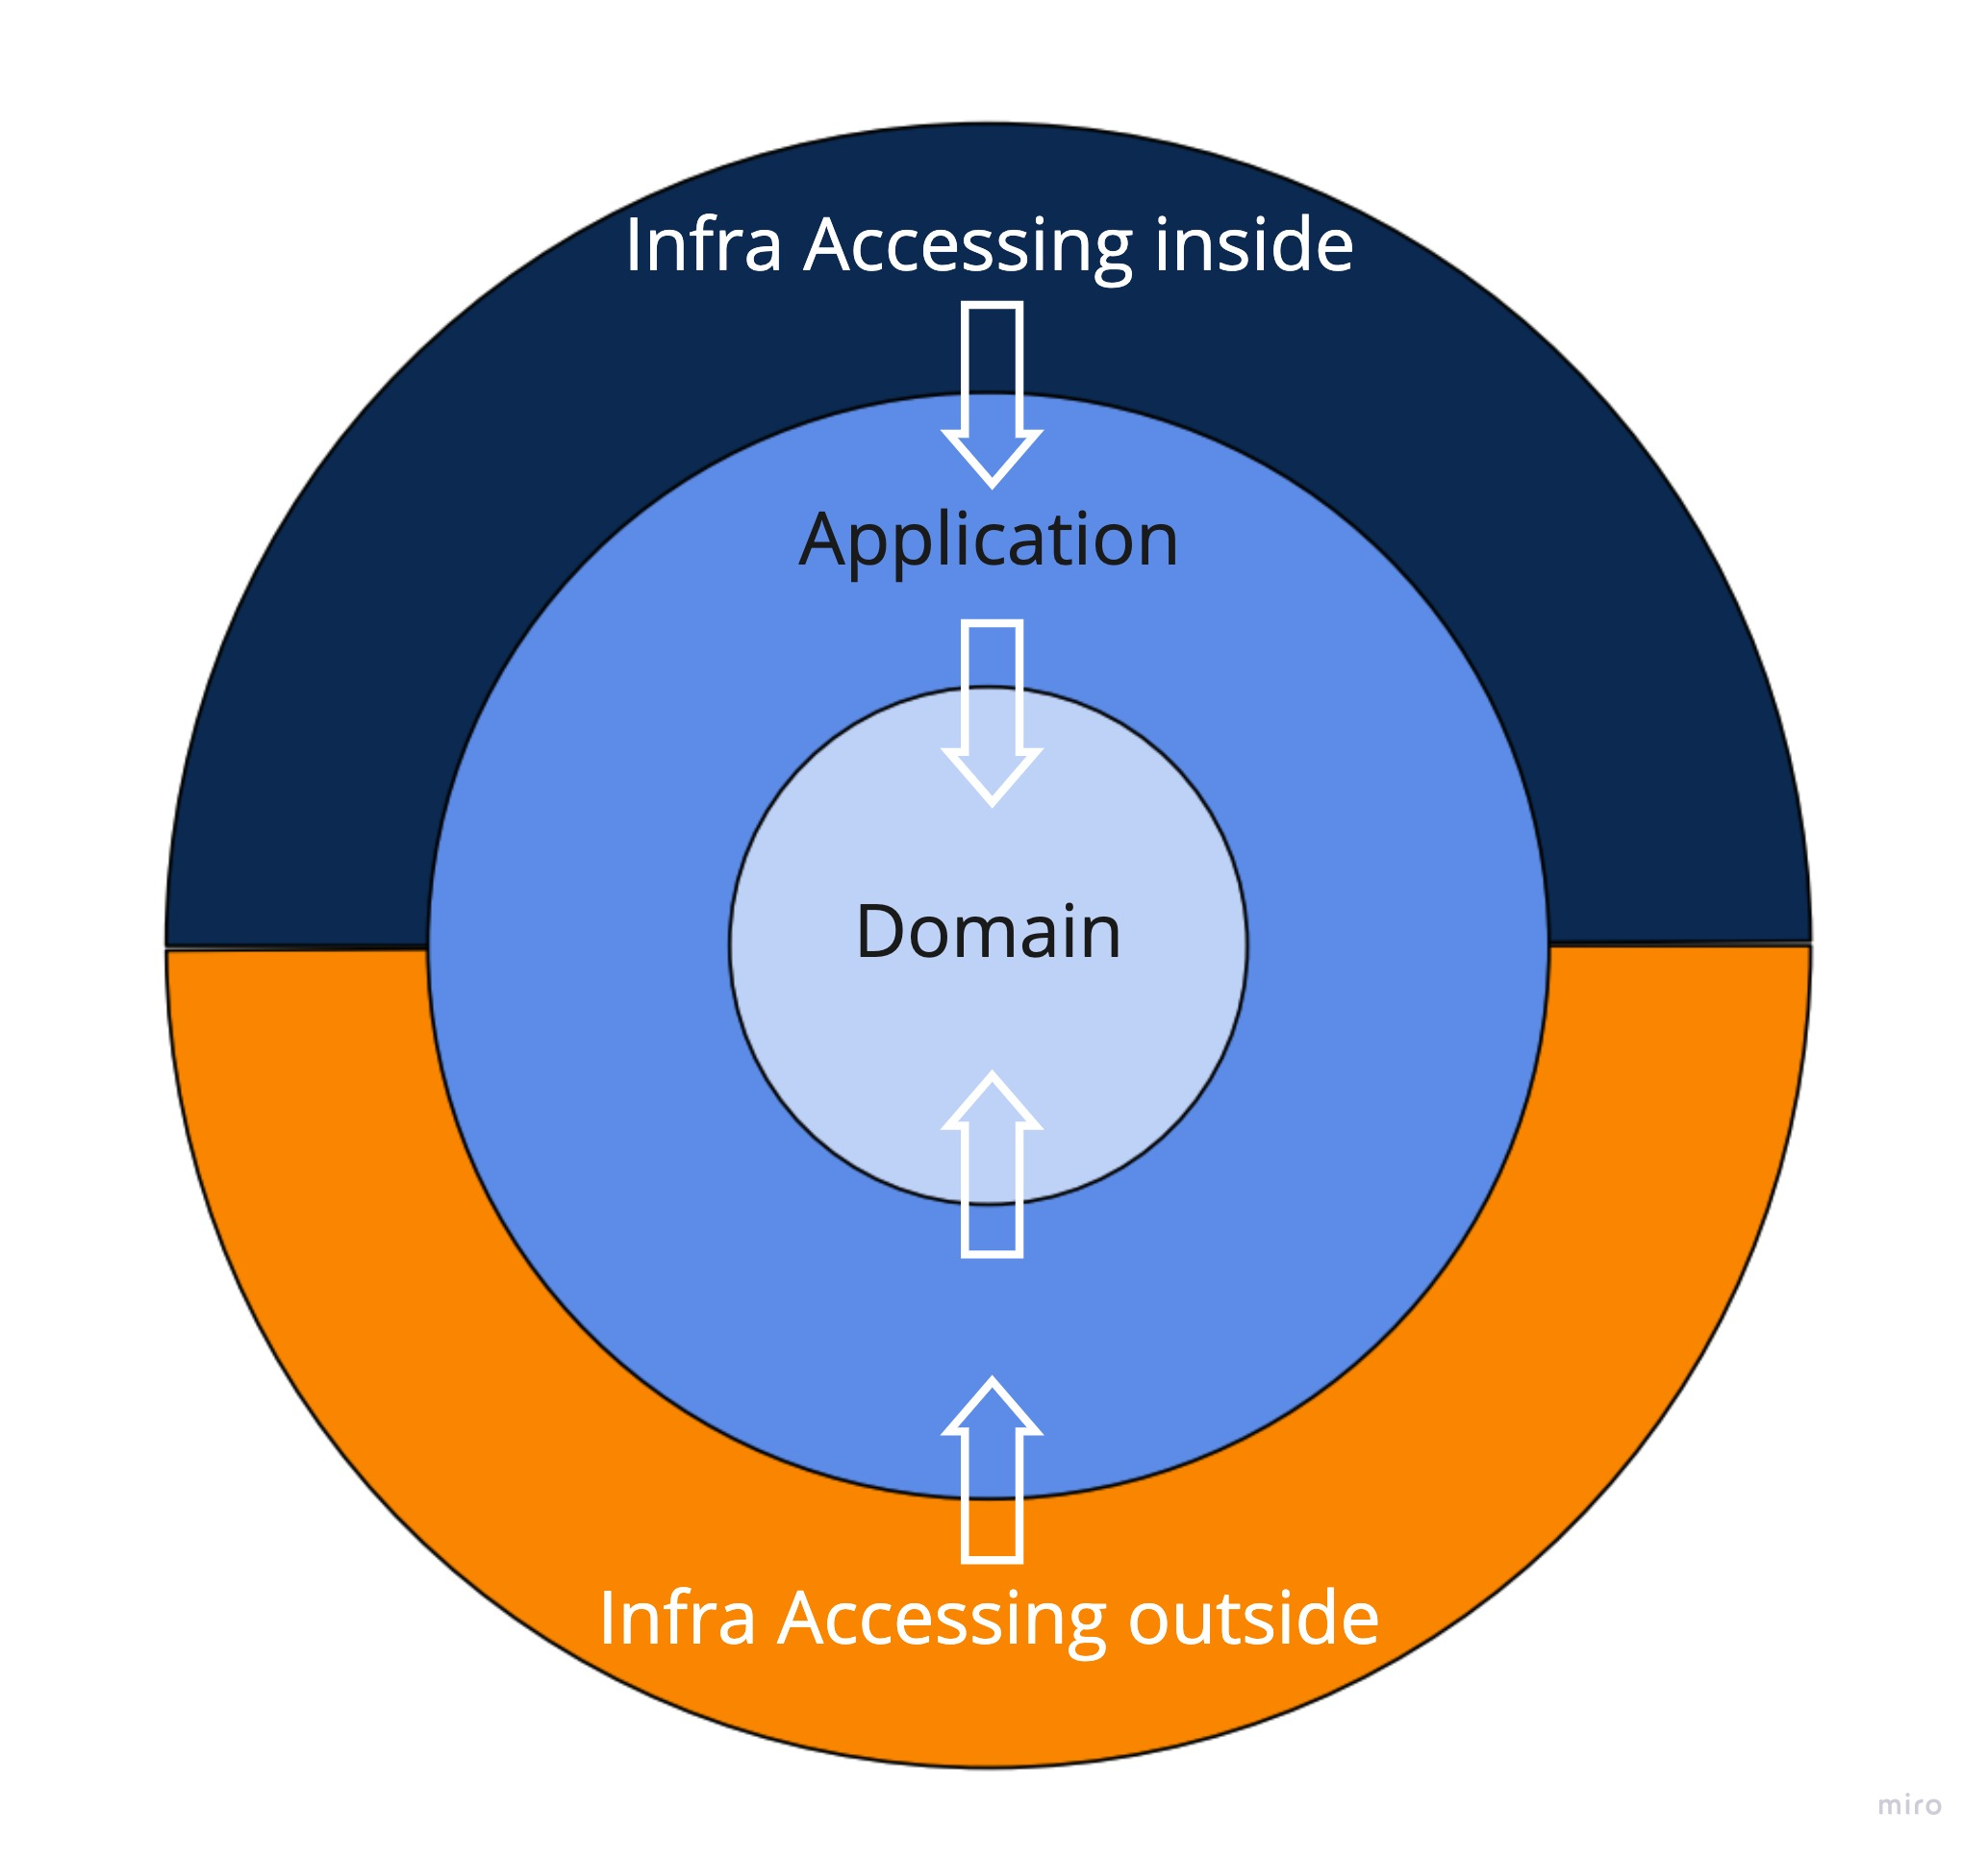
\includegraphics[height=0.3\textheight]{./part/Proyecto_ejecutivo/memoria_descriptiva/infoPreviaAntecedentes/img/PFM - Layer}
    \caption{layered architecture}\label{fig:layers}
\end{figure}

Junto con el concepto de arquitectura hexagonal y el\textit{DDD} vamos a aplicar el paradigma de diseño conocido como \gls{CQRS} (Command Query Responsibility Segregation). Es una técnica de diseño de arquitectura de software que separa la lógica de escritura (comandos) de la lógica de lectura (consultas) en sistemas de información. La idea es que las operaciones de escritura (comandos) y las operaciones de lectura (consultas) se manejen por separado, ya que tienen necesidades y características distintas. Mientras que las operaciones de escritura son responsables de modificar el estado de la aplicación, las operaciones de lectura son responsables de devolver información sobre ese estado sin modificarlo. Al separar estas dos responsabilidades, se pueden optimizar las operaciones de lectura para que sean más rápidas y escalables. Además, se puede diseñar una arquitectura de software más flexible, permitiendo una mayor adaptabilidad y evolución del sistema a medida que cambian los requisitos de la aplicación.

El resumen hasta ahora es que el diseño sigue una arquitectura hexagonal, con un enfoque\textit{DDD} en el dominio y un enfoque CQRS en los casos de uso. Es decir se diseñará un dominio rico y con un UL y se accederá a su funcionalidad a través de casos de uso que sigan el criterio de ser comandos y consultas.

El último detalle a explicar es cómo garantizar la separación efectiva de las capas en su uso de los elementos básicos con los que interactuan. Si un elemento de Infraestructura utiliza directamente una Entity de Dominio estaría saltando la capa de aplicación en su diagrama de dependencia. Bien es cierto que se mantendría la dependencia de fuera hacia adentro, pero se ha de tomar una decisión de hasta qué punto se quiere desacoplar una capa de otra. A esta decisión de diseño se le conoce como Estrategia de Mapping entre capas. Estrictamente cada capa requiere sus objetos de trabajo para estar desacoplada de las demás, pero como en todo aspecto de diseño está sometido a discusión acerca de seguir la teoría al pié de la letra y el pragmatismo de no verse envuelto en redundancias y sobredimensionar las soluciones.

En un extracto del libro Get Your Hands Dirty on Clean Architecture\cite{TomHombergs2019GYHD} podemos leer un extracto que es interesante rescatar ya que representa una conversación demasiado habitual entre compañeros de trabajo:

\textit{ The argument might have gone something like this:}

\begin{itemize}
    \item \textit{Pro-Mapping Developer:}
    \subitem  \textit{ If we don’t map between layers, we have to use the same model in both layers which means that the layers will be tightly coupled!}
    \item \textit{Contra-Mapping Developer:}
    \subitem \textit{ But if we do map between layers, we produce a lot of boilerplate code which is overkill for many use cases, since they’re only doing CRUD and have the same model across layers anyways!}
\end{itemize}
\textit{As is often the case in discussions like this, there’s truth to both sides of the argument. Let’s discuss some mapping strategies with their pros and cons and see if we can help those developers make a decision.}

Hay tantas estrategias como atajos dentro de este paradigma queramos asumir. Todo buen diseñador técnico debe saber tanto la teoría como los atajos que se pueden tomar. Evaluar los beneficios e inconvenientes y tomar una decisión con la que se ha de ser consecuente, y más importante en desarrollo, consistente. Esto quiere decir que una vez tomada una decisión debe ser una decisión en equipo que todos sigan. Es más eficiente un diseño imperfecto que sea consistente que un diseño perfecto en unos puntos e imperfecto en otros. Esto lleva al desorden a la hora de escribir código y complica la entrada de nuevos compañeros, el entendimiento del código existente con todas las consecuencias negativas que esto conlleva.

Los tipos de mapping que se documentan en este libro\cite{TomHombergs2019GYHD}:
\begin{itemize}
    \item The No Mapping Strategy~\cref{fig:nomapping}
    \item The Two-Way Mapping Strategy~\cref{fig:twowaymapping}
    \item The Full Mapping Strategy~\cref{fig:fullmapping}
    \item The One-Way Mapping Strategy~\cref{fig:onWaymapping}
\end{itemize}

Vamos a tomar diagramas del libro para entender cada estrategia. En todos los casos vemos simplificado el dominio a una única entidad, Account, y vemos como separa dicho dominio del acceso al caso de uso que envía dinero a una cuenta y del acceso a la infraestructura que guarda la información del envío de ese dinero.

\begin{figure}[H]
    \centering
    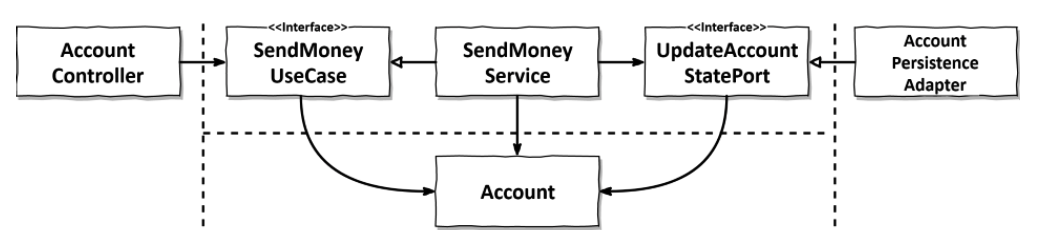
\includegraphics[height=0.1\textheight]{./part/Ejecucion/Seguimiento/CreateTaskUseCase/img/nomapping}
    \caption{No mapping strategy~\cite{TomHombergs2019GYHD}}\label{fig:nomapping}
\end{figure}

En la estrategia de No Mapping podemos ver en la figura~\cref{fig:nomapping} que tanto aplicación como Infraestructura dependen de Dominio. Esto evita todo código redundante, los \gls{DTO} (Data Transfer Object), pero resta flexibilidad. Si por detalles técnicos de una infraestructura concreta se requiere más o menos parámetros que los definidos en el Dominio o se deben guardar en otro formato que los definidos en Dominio enfrentaremos un problema.

\begin{figure}[H]
    \centering
    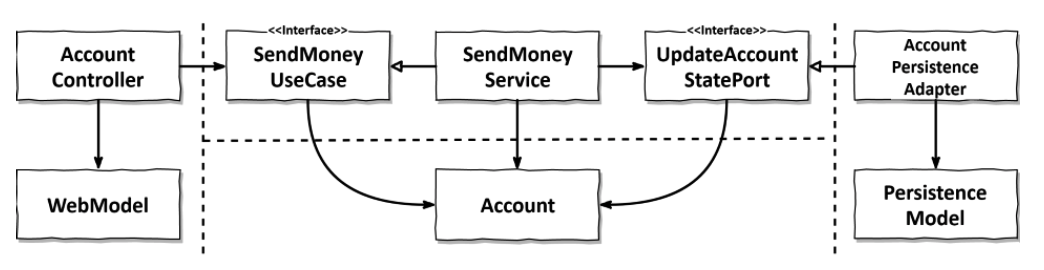
\includegraphics[height=0.1\textheight]{./part/Ejecucion/Seguimiento/CreateTaskUseCase/img/twowaymapping}
    \caption{two way mapping strategy~\cite{TomHombergs2019GYHD}}\label{fig:twowaymapping}
\end{figure}

En la estrategia de Two-Way Mapping Strategy~\cref{fig:twowaymapping} nos deshacemos de este problema y creamos un modelo DTO que sirva para transportar la información de una capa a otra necesaria para conformar la Entidad. De esta forma puede evolucionar por separado. Seguimos contemplando ese posible problema problema entre la Aplicación, los casos de uso, y el Dominio. Además tenemos que escribir más código para crear las entidades a través de los DTO y viceversa.

\begin{figure}[H]
    \centering
    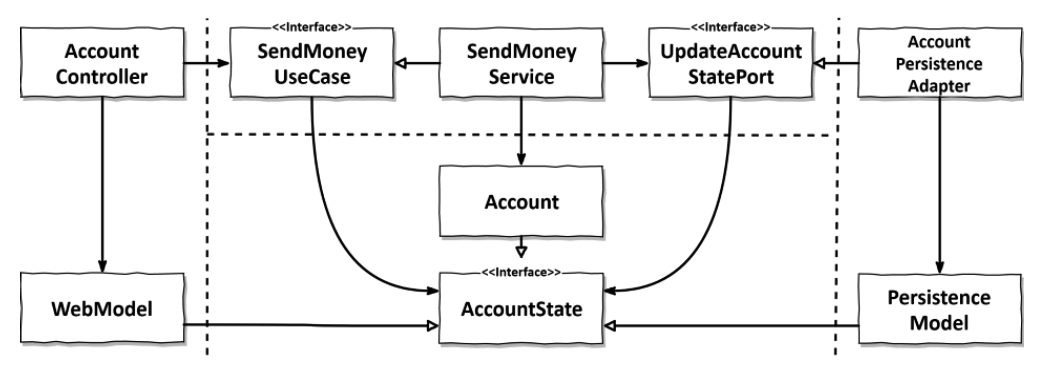
\includegraphics[height=0.1\textheight]{./part/Ejecucion/Seguimiento/CreateTaskUseCase/img/onWaymapping}
    \caption{One way mapping strategy~\cite{TomHombergs2019GYHD}}\label{fig:onWaymapping}
\end{figure}

En la figura de The One-Way Mapping Strategy~\cref{fig:onWaymapping} vemos que creamos una interfaz para la Entidad y hacemos depender de nuevo todas las capas de dicha interfaz. Se encuentran las capas más separadas y preparadas para el caso en el que se enfrente la necesidad de tener que crear distintas implementaciones aunque no se creen en un primer momento.

\begin{figure}[H]
    \centering
    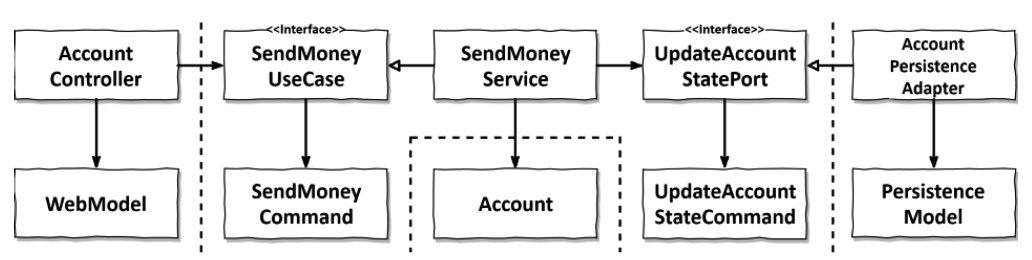
\includegraphics[height=0.1\textheight]{./part/Ejecucion/Seguimiento/CreateTaskUseCase/img/fullmapping}
    \caption{Full mapping strategy~\cite{TomHombergs2019GYHD}}\label{fig:fullmapping}
\end{figure}

En la figura de The Full Mapping Strategy~\cref{fig:twowaymapping} se opta por crear DTOs entre todas las capas. Es la solución más pura, pero el tradeoff es evidente: la cantidad de código a realizar es considerable y tiene que estar justificada con una necesidad de aislar hasta este punto.


No hay una regla de oro para elegir una estratégia que valga para todos los casos. Se reitera que debe ser una decisión de equipo, seguir la decisión todos y reevaluar con cada inconveniente que enfrente la decisión si se tiene que cambiar la estrategia.

Se puede ver el primer ejemplo en el un proyecto de ejecución que intentara resolver todas las decisiones y describir al detalle la solución a desarrollar no aportaría valor. Tomar una decisión de este tipo y documentarla, carece de utilidad porque no disponemos de información suficiente para tomar la decisión. Cuando nos enfrentamos al código es cuando podemos ver qué estrategia encaja mejor en nuestro caso.